
\chapter{Elements of PDE's}

Convergence was an interesting issue but the type of the equation we have to solve is also important. This is why we study the elements of the theory of PDE’s

\section{Quasi-linear equations – Conservative form}
A quasi-linear equation is an equation that is linear in the highest derivatives. We start with a first order equation. 

\subsubsection{General form of a first order quasi-linear equation in two variables}
We look for a function of $u(x,y)$ involving only first order derivatives in 2 space coordinates. And typically we have a linear combination of $x$ and $y$ derivatives and the coefficients may depend on $u$ too:

\begin{equation}
P(x,y,u) \frac{\D u}{\D x} + Q(x,y,u) \frac{\D u}{\D y} = R(x,y,u)
\label{2.1}
\end{equation}

This doesn't mean that the equation is linear, for example $\frac{\D u}{\D x} + u \frac{\D u}{\D y} = S(x,y,u)$: non linear Burger's equation. 

\subsubsection{General form of a second order quasi-linear equation in two variables}

The second order equation in 2 space variables is: 

\begin{equation}
\begin{aligned}
P\left(x,y,u, \frac{\D u}{\D x}, \frac{\D u}{\D y}\right) \frac{\D u^2}{\D x^2} &+ 2 S\left(x,y,u, \frac{\D u}{\D x}, \frac{\D u}{\D y}\right) \frac{\D u^2}{\D x \D y}\\
&+ T\left(x,y,u, \frac{\D u}{\D x}, \frac{\D u}{\D y}\right) \frac{\D u^2}{\D y^2} = H\left(x,y,u, \frac{\D u}{\D x}, \frac{\D u}{\D y}\right)
\end{aligned}
\end{equation}

In most applications in fluid mechanics, the factors multiplying the higher order derivatives do not depend explicitly on the independent variables $x,y$. But they will depend implicitly since $u$ is a function of $x,y$. Let's give an example of this, 2D potential equation for compressible flows: 

\begin{equation}
(a^2 - u^2)\frac{\D^2\varphi}{\D x^2} - 2uv \frac{\D ^2 \varphi}{\D x \D y} + (a^2 - v^2) \frac{\D ^2 \varphi}{\D y^2} = 0
\end{equation}

Quasi-linear equations can appears under the conservative/divergence form:

\begin{equation}
\frac{\D g_x}{\D x} + \frac{\D g_y}{\D y} (=\nabla .\vec{g}) = S(x,y,u)
\end{equation}

where $g_x, g_y = \vec{g}(x,y,u) = \vec{g}\left(x,y,u,\frac{\D u}{\D x}, \frac{\D u}{\D y}\right)$ for respectively a first order and a second order equation. Notice that it is possible to recover from here the quasi-linear form. Let's call $\tilde{g}_x (x,y) = \hat{g}_x(x,y,u(x,y))$, first order equation, then we have that by chain rule: 

\begin{equation}
\frac{\D \tilde{g}_x}{\D x} = \frac{\D \hat{g}_x}{\D x}  +\frac{\D \hat{g}_x }{\D u}\frac{\D u}{\D x} \qquad \frac{\D \tilde{g}_y}{\D y} = \frac{\D \hat{g}_y}{\D y}  +\frac{\D \hat{g}_y }{\D u}\frac{\D u}{\D y}
\end{equation}

Then the sum of the two gives: 

\begin{equation}
\begin{aligned}
\frac{\D \tilde{g}_x}{\D x} + \frac{\D \tilde{g}_y}{\D y} &= \frac{\D \hat{g}_x}{\D x} + \frac{\D \hat{g}_y}{\D y}  +\frac{\D \hat{g}_x }{\D u}\frac{\D u}{\D x} +\frac{\D \hat{g}_y }{\D u}\frac{\D u}{\D y}  \\
\frac{\D \hat{g} _x}{\D u} \frac{\D u}{\D x} + \frac{\D \hat{g}_y}{\D u} \frac{\D u}{\D y} &= S - \frac{\D \tilde{g}_x}{\D x} - \frac{\D \tilde{g}_y}{\D y}
\end{aligned}
\end{equation}

where we refined our coefficients $P$ and $Q$. For a first order equation in 2 space variables the converse is true as well. Indeed, defining $P= \frac{\D \hat{P}}{\D u}$ and $Q= \frac{\D \hat{Q}}{\D u}$, the chain rule is: 

\begin{equation}
\frac{\D \tilde{P}}{\D x} = \frac{\D \hat{P}}{\D x}  +\frac{\D \hat{P}}{\D u}\frac{\D u}{\D x}= \frac{\D \hat{P}}{\D x} + P\frac{\D u}{\D x} \qquad \Rightarrow P\frac{\D u}{\D x} = \frac{\D \tilde{P}}{\D x} - \frac{\D \hat{P}}{\D x}
\end{equation}

Replacing these in the general first order equation form \eqref{2.1}, we find back the conservative form: 

\begin{equation}
\frac{\D \tilde{P}}{\D x} + \frac{\D \tilde{Q}}{\D y} = S + \frac{\D \hat{P}}{\D x} + \frac{\D \hat{Q}}{\D y}
\end{equation}

For a second order equation, this is not always possible. 

\section{Characteristic surfaces and wave-like solutions}
\subsection{First order scalar equation in m independent variables}

It means that we have a linear combination such as: 

\begin{equation}
a_i \frac{\D u}{\D x_i} = 0 
\label{2.9}
\end{equation}

For simplicity we take the source term $=0$. We suppose to solve an initial value problem (Cauchy problem). We imagine that the solution is known on some hyper-surface $S^*$ (in 2D a curve) of equation $F(x_i) = 0$. Does this problem have one and only one solution? \\

The value of $u$ on the surface is called the \textbf{trace} of the solution on the hyper surface and it is specified. Imagine that we can construct a function $\varphi (x,y)$ such that it is equal to $u$ on the surface. Typically if we think in 2D, we specify $u$ on a curve and we elongate it arbitrarily. Because the function $\varphi = u$ on the surface, then the tangential derivative of $\varphi$ and $u$ are the same. If we construct the function $\varphi - \lambda F$ is also equal to $u$ on the surface whatever the value of $\lambda$. In other words, I know u on the curve, I construct a function $\varphi$ and then I say that all the function $\varphi - \lambda F$ are the same as $u$, so we have an infinite number of solution on the surface. But there exists one $\lambda$ for which the normal derivative will be the same as the normal derivative of $u$: 

\begin{equation}
\nabla \varphi - \lambda \nabla F = \nabla u \qquad \Leftrightarrow \frac{\D \varphi}{\D x_i } - \lambda \frac{\D F}{\D x_i } = \frac{\D u}{\D x_i} \quad i = 1,\dots, m
\end{equation} 

The unknowns in this equation are the partial derivatives of $u$ but are given by $a_i \frac{\D u}{\D x_i} = 0$. We have thus a system of $m+1$ equations and $m+1$ unknowns. The system can be put under matrix form as:

\begin{equation}
\left(
\begin{array}{ccccc}
1 & \dots & & & \frac{\D F}{\D x_1} \\
 & 1 &  & & \frac{\D F}{\D x_2}\\
 \vdots & & & & \vdots \\
 a_1 & a_2 & \dots & a_m & 0
\end{array}
\right)
\left(
\begin{array}{c}
\frac{\D u}{\D x_1}\\
\vdots\\
\frac{\D u}{\D x_m}\\
\lambda
\end{array}
\right)
=
\left(
\begin{array}{c}
\frac{\D \varphi}{\D x_1}\\
\vdots\\
\frac{\D \varphi}{\D x_m}\\
0
\end{array}
\right)
\end{equation}

The system has one and only one solution unless if the determinant is equal to 0, unless the surface S is such that $a_i \frac{\D F}{\D x_i} = 0 = \vec{a}.\nabla F$. In fact $\nabla F$ is parallel to the normal to the surface because all the tangential derivatives are 0 and the only component that cannot be 0 is the normal derivative, so $\nabla F \propto \vec{n}$. And if we say $\vec{a}.\vec{n} = 0$,
this means that the surface is tangent to $\vec{a}$. These $\vec{a}$ are called \textbf{characteristic lines} of a \textbf{characteristic surface}. The response to the question is thus that yes the solution is unique unless if the surface is a characteristic surface for which case we have no solution or an infinity of solutions if compatible. In 2D this is a characteristic curve. \\

The original equation \eqref{2.9} admits solutions of the form: $u = \hat{u}\exp (IF(x_i))$ where $F(x_i) = 0$ are equations of characteristic surfaces. Because if we compute $\frac{\D u}{\D x_i} = I u \exp (IF(x _i))\frac{\D F}{\D x_i} = Iu\frac{\D F}{\D x_i}$ and thus 

\begin{equation}
a_i \frac{\D u }{\D x_i} = IU a_i \frac{\D F}{\D x_i}=0
\end{equation}

which is identically satisfied if $\vec{a}.\vec{n} = 0$. Lines of constant $F$ are wave fronts of wave-like solutions since we have $\exp (I F(x_i))$ similar to $\exp (kx - \omega t)$. A special case is when $a_i = cst \rightarrow \frac{\D F}{\D x_i = n_i}$ where we have planar wave that propagates without dilatation or damping ($\hat{u}=cst$).  

\subsection{Second order equations in one unknown in two dimension}
Consider the second order equation in two variables:

\begin{equation}
R\frac{\D ^2 u}{\D x^2} + 2S \frac{\D ^2 u}{\D x\D y} + T \frac{\D ^2 u}{\D y^2} = 0
\end{equation}

In this case we have to provide $u$ and $\nabla u$ but if we know the surface we can compute $\nabla u$. Let's call $p = \frac{\D u}{\D x}$ and $q = \frac{\D u}{\D y}$ on the curve. Let's call $\varphi$ a function equal to $p$ on C. It results that $\varphi = p + \lambda F$ on C and therefore there exists a value of $\lambda$ such that $\nabla \varphi = \nabla p + \lambda \nabla F$. So we have also for the second variable: 

\begin{equation}
\psi = q + \mu F \qquad \Rightarrow \nabla \psi = \nabla q + \mu \nabla F
\end{equation}

The unknowns are $\lambda , \mu$, the components of the gradients $p$ and $q$. But we know that 

\begin{equation}
\nabla p = \frac{\D ^2 u}{\D x^2} \vec{e}_x + \frac{\D ^2 u}{\D x \D y} \vec{e}_y\qquad \nabla q = \frac{\D ^2 u}{\D y^2} \vec{e}_y + \frac{\D ^2 u}{\D x \D y} \vec{e}_x
 \end{equation}
 
Again we have a system of equation

\begin{equation}
\left( 
\begin{array}{ccccc}
1 & 0 & 0 & \frac{\D F}{\D x} & 0\\
0 & 1 & 0 & \frac{\D F}{\D y} & 0 \\
0 & 1 & 0 & 0 & \frac{\D F}{\D x} \\
0 & 0 & 1 & 0 & \frac{\D F}{\D y} \\
R & 2S & T & 0 & 0
\end{array}
\right)
\left( 
\begin{array}{c}
\frac{\D p}{\D x} \\
\frac{\D p}{\D y} = \frac{\D q}{\D x}\\
\frac{\D q }{\D y}\\
\lambda\\
\mu 
\end{array}
\right)
=
\left( 
\begin{array}{c}
\frac{\D \varphi}{\D x} \\
\frac{\D \varphi}{\D y} \\
\frac{\D \psi}{\D x}\\
0\\
0
\end{array}
\right)
\end{equation}

If we try to compute the determinant we will get 

\begin{equation}
\det = R \frac{\D F}{\D x} \left( - \frac{\D F}{\D x} \right) - 2 S \frac{\D F}{\D x}\frac{\D F}{\D y}  +T \left( -\frac{\D F}{\D y}\right)\frac{\D F}{\D y} = - \left(\frac{\D F}{\D y}\right) ^2 \left[ Rz^2 + 2 Sz 
+ T \right]
\end{equation}

where $Z = \frac{\frac{\D F}{\D x}}{\frac{\D F}{\D y}} = \frac{n_x}{n_y}$. The line $F(x,y) = 0$ is a characteristic line when $Rz^2 + 2Sz + T = 0$. If $S^2 - RT > 0$ so we have 2 roots and thus 2 characteristic directions at each point. In the case $S^2 - RT < 0$ we have no real root no characteristic line for this equation. And if $S^2 - RT = 0$ we have 2 identical roots so 1 characteristic direction. If now we have a quadratic term like 

\begin{equation}
R x^2 + 2S xy + Tx^2 = 0
\end{equation}

The first case would give a hyperbole, the second an elliptic equation and the last we have a parabolic equation. 

\subsubsection{Applicaition: potential flow equation}

\begin{equation}
\begin{array}{c}
R = a^2 - u^2 \qquad S = -uv \qquad T = a^2 - v^2 \\ 
\Rightarrow S^2 - RT = u^2v^2 - (a^2 -u^2)(a^2 - v^2) = a^2 [u^2 + v^2 - a^2] = a^4 \left[M^2 - 1 \right]
\end{array}
\end{equation}

We can see that when $M>1$ hyperbolic, $M = 1$ parabolic, $M<1$ elliptic, the parameters $R,S,T$ change size within the domain. 

\subsection{System of first order equations in two dimensions}
We can write it in the form of a system of n equations and n unknowns:

\begin{equation}
A_x \frac{\D U}{\D x}  +A_y \frac{\D U}{\D y} = 0
\end{equation}

It is now $U$ that is provided on the curve C of equation $F(x,y) = 0$. We call $V$ a vector function which is identical to $U$ on C. We are going to have a vector of Lagrange multipliers $\Theta$: 

\begin{equation}
V = U + \Theta F \mbox{ on C} \qquad \Rightarrow \frac{\D V}{\D x} = \frac{\D U}{\D x} + \Theta \frac{\D F}{\D x} \qquad \frac{\D V}{\D y} = \frac{\D U}{\D y} + \Theta \frac{\D F}{\D y}
\end{equation}

We will again have the matrices: 

\begin{equation}
\left( 
\begin{array}{ccc}
I & 0 & \frac{\D F}{\D x}I\\
0 & I & \frac{\D F}{\D y} I\\
A_x & A_y & 0
\end{array}
\right)
\left(
\begin{array}{c}
\frac{\D U}{\D x}\\
\frac{\D U}{\D y}\\
\Theta
\end{array}
\right)
=
\left(
\begin{array}{c}
\frac{\D V}{\D x}\\
\frac{\D V}{\D y}\\
0
\end{array}
\right)
\end{equation}

Again we have to compute the determinant. The characteristic directions are $|A_x n_x + A_y n_y| = 0$ and if we factorize: 

\begin{equation}
n_x |A_x + \tilde{\lambda} A_y| = 0 \qquad n_y \left|-A_x \frac{-n_x}{n_y} + A_y\right| = 0
\end{equation} 

where $\frac{-n_x}{n_y}$ is the slope of the tangent to the characteristic lines. We end up with an eigenvalue problem

\begin{equation}
|A_y - \lambda A_x| = 0
\end{equation}

if $\det (A_x) \neq 0$ so $|A_y - \lambda A_x| = |A_x||A_x^{-1}A_y - \lambda I| = 0$. We have n real roots, n lin indep real eigenvectors (hyperbolic) or n real roots, m<n lin indep real eigenvectors (parabolic)\footnote{This is what happens when all derivatives of one component of U with respect to one independent variable x or y are missing.}. We also have the case elliptic problem with n complex roots. Other possibilities (complex + real roots) = hybrid, as previous mixed problems. \\

Notice that if we if we denote $\Lambda$ the diagonal matrix of eigenvalues and $L$ the matrix of left (line) eigenvectors, we can write: 

\begin{equation}
L(A_y - \lambda A_x) = 0 \Leftrightarrow LA_y - \Lambda LA_x = 0 \qquad \Rightarrow LA_x \frac{\D U}{\D x} + LA_y \frac{\D U}{\D y} = 0 \Leftrightarrow \frac{\D W}{\D x} + \Lambda \frac{\D W}{\D y} = 0 
\end{equation}

In the case of second order equations we would have: 

\begin{equation}
\begin{aligned}
R\frac{\D ^2 u}{\D x^2} + 2S \frac{\D ^2 u}{\D x \D y} + T\frac{\D ^2 u}{\D y^2} = 0 \qquad &\Leftrightarrow R\frac{\D p}{\D x}  + S \left(  \frac{\D p }{\D y	} + \frac{\D q}{\D x}\right) + T\frac{\D q}{\D y} = 0\\
\left[
\begin{array}{cc}
R & S\\
0 & 1
\end{array}
\right]
\frac{\D }{\D x}\left( 
\begin{array}{c}
p\\
q
\end{array}
\right)
&+ \left( 
\begin{array}{cc}
S & T\\
1 & 0
\end{array}
\right)\frac{\D q}{\D x} - \frac{\D p }{\D y} = 0
\end{aligned}
\end{equation}


\subsection{Systems of n equations in m independent variables}
In that case the generalization is: 

\begin{equation}
A_i \frac{\D U}{\D x_i} = 0
\end{equation}

where $A$ is n by n matrix and $U$ a n by 1 vector. The equations for the characteristic surfaces are now: 

\begin{equation}
|A_i n_i| = 0
\end{equation}

We have again an eigenvalue problem, but it differs from previous ones since among the m components of $\vec{n}$, $m-1$ can be chosen arbitrarily, defining the nature of the problem, relatively to the variable associated to the component to determine. It will be respectively hyperbolic, parabolic, elliptic or hybrid if it is so for all the directions in the subspace of dimension $m-1$. \\

In general, if the problem is hyperbolic wrt one variable, it is indeterminate wrt the other variables, this is due to the fact that the component to be determined takes value in an interval wrt the first variable. As the problem admits wavelike solutions it can be named hyperbolic. Since for unsteady problems time often plays the role of privileged variable, it is common to designate the variable for which the problem is hyperbolic as \textbf{time-like} variable. In contrast, a problem elliptic wrt one variable is also for the others. 

\exemple{
To illustrate suppose that we have: 

\begin{equation}
|A_x n_x + A_yn_y + A_zn_z | = 0
\end{equation}

We can write this in the following way: 

\begin{equation}
\left|\frac{A_x n_x + A_y n_y}{n_z } + A_z\right| = 0 \qquad \Rightarrow \left|\frac{A_x n_x + A_y n_y}{\sqrt{n_x^2 + n_y^2}}- \frac{\sqrt{n_x^2 + n_y^2}}{n_z} + A_z\right| = 0
\end{equation}

where in fact the first term is the direction of $n$ and the second term plays the role of the previous $\lambda$. If it is in 4D, we would have 2 angular directions defining the $n$ direction. $m-2$ variables can be chosen arbitrarily and the last is given by the eigenvalue problem. The system is hyperbolic wrt to $A_z$ if the eigenvalues are all real and we have a complete set of eigenvectors for all directions whatever the direction. If in contrast they are all complex whatever the direction, it is indetermined. The Euler equations will be: 

\begin{equation}
\frac{\D U}{\D t } + \frac{\D F}{\D x} = 0 \qquad 
U = \left(
\begin{array}{c}
\rho \\
\rho u\\
\rho E
\end{array}
\right)
\quad F = \left(
\begin{array}{c}
\rho u\\
p + \rho u 2\\
\rho uH
\end{array}
\right)
\end{equation}

in 1D unsteady, z is an independent variable. We also know that $p = \rho RT = \rho (c_p - c_v) T$ and $z = c_v T = \rho (\gamma -1)c_v T$ and $p =\rho (\gamma -1)e, E = e+\frac{u^2}{2}, H = E + \frac{p}{\rho}$, so that we have: 

\begin{equation}
\frac{\D F}{\D U} = \left( 
\begin{array}{ccc}
0 & 1 & 0\\
\frac{\D p}{\D e} - u^2 & 2u + \frac{\D p}{\D \rho u} & \frac{\D p}{\D \rho E}\\
\times & \times & \times
\end{array}
\right)
\end{equation}

And we see that the eigenvalues are real: $u+a, u , u-a$. In 2D the $U$ and $F$ vectors are $4\time 1$ and thus the matrix will be $4\times 4$ : 

\begin{equation}
\begin{aligned}
&2D: \quad \frac{\D U}{\D t} + \frac{\D F_x}{\D x}+ \frac{\D F_y}{\D y}  = 0\\
&3D: \quad \frac{\D U}{\D t} + \frac{\D F_x}{\D x}+ \frac{\D F_y}{\D y} + \frac{\D F_z}{\D z}  = 0
\end{aligned}
\end{equation}

They are both unsteady with 3 and 4 independant variables. We see that these are hyperbolic wrt the time variable!} 

\ \\

\theor{
\textbf{Conclusion}\\

If the system has real eigenvalues and a complete set of real eigenvalues for all values of the arbitrary parameters (m-2) $\rightarrow$ the system is hyperbolic wrt the variable of interest $\rightarrow$ this variable plays a special role, it is the evolution or time-like variable. \\

If the system has only complex eigenvalues the equation is elliptic. In that case, it is generally elliptic wrt all variables. 
}

\subsection{Notion of well posed problem}
Problem that has one and only one solution, depending continuously on the prescribed initial/boundary data. The last condition is primordial, if the initial conditions vary infinitesimally, the solution may only vary infinitesimally.  The initial conditions choice will define if the problem is well or ill-posed. The way to define them vary with the type of the problem. Let's illustrate with Laplace's equation: 

\begin{equation}
\frac{\D ^2 u}{\D x^2} + \frac{\D ^2 u}{\D y^2} = 0
\end{equation}

and we compute the solution on the domain $\Omega$ which is the right half plane where $x\geq 0$. The boundary of the domain is $u(0,y) = 0$ and $\frac{\D u}{\D x}(0,y) = h(y)$. Since it is elliptic equation it has no real characteristic curve so we know that the curves are not characteristic and so that we have one and only one solution. If we take: 

\begin{equation}
h(y) = 0 \Rightarrow u=0 \qquad h(y) = \frac{\sin ny}{n} \Rightarrow u = \frac{1}{n^2}\sinh nx \sin ny
\end{equation}

As $n\rightarrow \infty, h \rightarrow 0$, but for any non-zero $x$ the solution will vary a lot. When we are never sure that the solution depends continuously on the boundary condition and when we have uncertainties on the boundary conditions we can never be sure of the solution. This is why if we have 2 boundary we have to impose one condition on each boundary. 

\section{Properties of hyperbolic equations}
\subsection{Nature of the solution - Riemann invariants}
For simplicity, consider a system of n first order equations in 2 independent variables $|A_x n_x + A_y n_y| = 0 \Leftrightarrow |A_y - \lambda A_x| = 0$ where $\lambda = -n_x/n_y$. If $A_x$ is positive definite regular matrix: 

\begin{equation}
|A_x (A_x^{-1}A_y - \lambda I)| = 0 \qquad \Rightarrow |A_x||\underbrace{A_x^{-1}A_y}_{A}-\lambda I| = 0
\end{equation}

The $\lambda _s$ are the eigenvalues of $A$. With $|A-\lambda I|v = 0 \Rightarrow Av = \lambda v$ where $v$ are the right eigenvectors and $l$ the line eigenvectors: $lA = \lambda l \Leftrightarrow (lA)^t = \lambda l^t$. We have the following algebraic identities: 

\begin{equation}
Av_1 = \lambda _1v_1 \quad Av_2 = \lambda _2v_2 \dots \qquad \Rightarrow A R = R \Lambda \Leftrightarrow R^{-1}AR = \Lambda \Leftrightarrow R^{-1} A = \Lambda R^{-1}
\end{equation}

We find the relation $L = R^{-1}$. Let's imagine that the initial problem to solve is (as in aerodynamics course - Riemann): 

\begin{equation}
A_x \frac{\D U}{\D x} + A_y \frac{\D U}{\D y} = S\qquad \Leftrightarrow  \frac{\D U}{\D x} + A \frac{\D U}{\D y} = \underbrace{A_x^{-1} S}_G \Leftrightarrow L\frac{\D U}{\D x} + \Lambda L \frac{\D U}{\D y} = LG
\end{equation}

If now we expand first line: 

\begin{equation}
\begin{aligned}
l_{11} \frac{\D u_1}{\D x} + l_{12} \frac{\D u_2}{\D x} + \dots + l_{1n} \frac{\D u_n}{\D x} + \lambda_1 &\left[ l_{11} \frac{\D u_1}{\D y} + \dots \right] = (LG)_1 \\
l_{11} \frac{\D u_1}{\D x} + \lambda_1 l_{11} \frac{\D u_1}{\D y} = l_{11} \left( \frac{\D u_1}{\D x} + \lambda_1 \frac{\D u_1}{\D y}\right) &= l_{11} \left( \frac{\D u_1}{\D x} + \tan \theta \frac{\D u_1}{\D y}\right) \\
&= \frac{l_{11}}{\cos \theta} \left(\cos \theta \frac{\D u_1}{\D x} + \sin \theta\frac{\D u_1}{\D y}\right)
\end{aligned}
\end{equation}

where $\frac{1}{\cos \theta} = \sqrt{1+\lambda ^2}, \vec{e}_\theta .\nabla u = \frac{du_1}{ds_1}$ (directional derivative in the characteristic direction with slope $\lambda _i$). This can be done for every indexes and we get: 

\begin{equation}
\frac{1}{\cos \theta} \left( l_{11} \frac{du_1}{ds_1} + \dots + l_{1n}\frac{du_n}{ds_1} \right) = h_1
\end{equation}

For a system of n equations, the system transforms into a system of n ordinary differential equations: 

\begin{equation}
l_{ij} \frac{d u_j}{ds_{i}} = h_i \cos \theta _i = \frac{h_i}{\sqrt{1+\lambda ^2_i}}
\end{equation} 

This is a set of ordinary differential equtions along the characteristic curve $i$. Can we simplify further? If $l_{ij}$ do not depend explicitly on the independent variables $x,y$ (they depend only on $u_j$, true when $A$ does not depend on $x,y$), there may exist a function $f(u_j)$ (integrating factor) such that 

\begin{equation}
fl_{ij} \frac{du_j}{ds_i} = \frac{dR_i}{ds_i}
\end{equation}

The left hand side is an exact differential of a certain function $R_i$. With the conditions: 

\begin{equation}
fl_{ij} = \frac{\D R_i}{\D u_j} \Rightarrow \frac{\D fl_{ij}}{\D u_k} = \frac{\D fl_{ik}}{\D u_j} \qquad fl_{ik} = \frac{\D R_i}{\D u_k}
\end{equation}

\wrapfig{14}{l}{6}{0.3}{ch2/1}
$f$ is called an integrating factor. If $n\leq 2\rightarrow f$ always exists, if $l_{ij}$ are constant $\forall n, R_i = l_{ij} u_j$ and if the system is homogeneous $g_i = 0 \rightarrow h_i = 0 \ \forall i$ we have: 

\begin{equation}
\frac{d R_i}{ds_i} = \frac{f h_i}{\sqrt{1+\lambda ^2_i}} = 0 \qquad \Rightarrow R_i = cst
\end{equation}

$R_i$ are the characteristic variables. The characteristic variables in previous section were the component of the vector $W = LA_yU$. When these are constant over a characteristic curve, they are called \textbf{Riemann invariants}. The summary is given on the figure. 

Let's try to think about the properties of the solution. We restrict to the case of a system of two equations in 

\wrapfig{8}{r}{4}{0.3}{ch2/2}
two unknowns (so 2 characteristics). The solution is prescribed on the curve $\Gamma$, the solution at point P has to depend on all the solutions on the characteristic (integration) but these depend on the value of the solution in the section APB. In conclusion, the dark area is called the \textbf{region of dependence} of P. An analogous reasoning can denote the region behind P as \textbf{zone of influence of P}. The rest of the region is the \textbf{zone of silence}. 

\subsection{Well-posed problem for a hyperbolic system}
The previous discussion allows to state that the Chauchy problem is well-posed for hyperbolic equations. Indeed, since the solution at point P only depends on the values of the solution upstream this point, we can compute it everywhere downstream of $\Gamma$. Furthermore, if the initial data are perturbed infinitesimally, the solution at any point will be perturbed so since wave-like solutions (property of hyperbolic equations) propagate without amplification or damping. As the solution is computed by progressing in the domain, the problem is an \textbf{evolution problem}. Unsteady (time dependent) physical problems always lead to evolution problems. It is customary to note $t$ the time-like variable with respect to which the problem is hyperbolic. Often the curve or surface over which the values of the dependent variables are specified is the surface $t=t_0$ and they are called initial conditions ($\rightarrow$ initial value problem).\\
 
Consider 1D inviscid compressible flow in a tube of length $L$. Continuity, x-momentum and energy equations tells that: 

\begin{equation}
\frac{\D \rho}{\D t} + \frac{\D \rho u}{\D x} = 0 \qquad \rho \frac{\D u}{\D t} + \rho u \frac{\D u }{\D x} = - \frac{\D p}{\D x}= -a^2\frac{\D \rho}{\D x} \qquad \dot{s} = 0
\end{equation}

If initial data are homentropic (uniform initial entropy): $s = cst$. We can rewrite: 

\begin{equation}
\begin{aligned}
&\frac{\D \rho}{\D t} + \frac{\D \rho u}{\D x} = 0 \qquad \frac{\D u}{\D t} + u \frac{\D u }{\D x} + \frac{a^2}{\rho} \frac{\D \rho}{\D x} = 0\\
\Rightarrow &\frac{\D }{\D t} \left( 
\begin{array}{c}
\rho \\
u
\end{array}
\right) + \left( 
\begin{array}{cc}
u & \rho\\
\frac{a^2}{\rho} & u
\end{array}
\right) 
\frac{\D}{\D x} \left( 
\begin{array}{c}
\rho \\
u
\end{array}
\right) 
=
\left( 
\begin{array}{c}
0 \\
0
\end{array}
\right) 
\end{aligned}
\end{equation}

\wrapfig{8}{l}{5}{0.3}{ch2/3}
The eigenvalues of $A$ are $\lambda = u\pm a$, confirming that it is hyperbolic. If we make the drawing, we have the graph of x in function of t and since the region of influence of the left boundary is limited to the triangle, we have to specify the upper and lower boundary conditions to be able to compute in all the tube. We have to supply as many information as the number of characteristic curves entering the domain, there is one on down boundary and one on top so we can prescribe the velocity for example. \\

\subsection{Non-linear equations – Weak solutions}
Consider the advection/reaction equation without source term: 

\begin{equation}
\frac{\D u}{\D t} + u \frac{\D u}{\D x} = 0
\end{equation}

Characteristic curves are lines tangent to the vector $\vec{a} = \vec{e}_t + u \vec{e}_x$, with slope $u$. Along the characteristics $\frac{\D u }{\D t} + u \frac{\D u }{\D x} = \sqrt{1+\lambda ^2} \frac{d u}{ds}$. The Riemann invariant is $u = cst$ on the curves. The equation of the characteristics are $x = x_0 + u t$ and the general solution of the homogeneous equation is $u = f(x-ut)$. The slope of the characteristics depend on the solution, it is possible that the lines cross. In that case on which curve do we have to rely to find the solution? \\

\wrapfig{8}{r}{6}{0.4}{ch2/4}
Consider the figure with the boundary conditions $A,B$, two cases can happen $A<B, A>B$. In the first case, the characteristics don't cross and an empty region appears, that can be filled by a \textbf{fan} $u = x/t$. In the second case, the characteristics cross. In that case the solution is not uniquely defined since it has to take both value A and B. The equation does not have a solution in the strong form. The weak form of the problem is:  

\begin{equation}
\int _0 ^\infty dt \int _{-\infty}^\infty \nu \left[\frac{\D u}{\D t} + u \frac{\D u }{\D x}\right] dx = 0 
\end{equation}

Then we can integrate by part and find that: 

\begin{equation}
\begin{aligned}
\int \int \nu \left[ \frac{\D u}{\D t} +\frac{\D u^2/2}{\D x}\right] dx\, dt &= \int \int \left[ \frac{\D uv}{\D t} + \frac{\D}{\D x} \frac{u^2}{2} \nu  \right]dx\, dt - \int \int \left[ u\frac{\D \nu}{\D t} + \frac{u^2}{2}\frac{\D \nu }{\D x}\right]dx\, dt  =0 \\
&=-\int _0^\infty  \int _{-\infty}^\infty \left[u \frac{\D \nu}{\D t} + \frac{u^2}{2}\frac{\D \nu }{\D x}\right] dx\, dt = -\int _{-\infty}^\infty u(0,x)\nu (0,x) \, dx
\end{aligned}
\end{equation}

This form allows discontinuities, the question is now where are they located? For this let's consider the integral of the strong form: 

\begin{equation}
\frac{d}{dt} \int _{x_1}^{x_2} u \, dx + \left[ \frac{u^2}{2}\right]_{x_1}^{x_2} = 0 
\end{equation}

and let's assume that there exists a discontinuity between $x_1$ and $x_2$ (jump from A to B). We can thus note $x_s$ the location of the discontinuity and $\int _{x_1}^{x_2} = (x_s - x_1)A + (x_2 - x_s)B$ such that: 

\begin{equation}
\frac{d}{dt} \int _{x_1}^{x_2} u \, dx = (A- B)\frac{d x_s}{dt} \equiv (A - B) \dot{x}_s
\end{equation}

where $\dot{x}_s$ is the discontinuity displacement velocity. We can reconsider the equation noticing: 

\begin{equation}
\dot{x}_s (B-A) = \left[ \frac{u^2}{2} \right]_{x_1}^{x_2} = \frac{B^2 - A^2}{2} \qquad \Rightarrow \dot{x}_s = \frac{A + B}{2}
\end{equation}

It is this solution which is represented on figure (b). This result is completely general for a general equation in the form: 

\begin{equation}
\frac{\D u}{\D t} + \frac{\D f(u)}{\D x} = 0
\end{equation}

\theor{
The jump is called shock and the states on both side of the shock and the shock speed are linked by the jump condition also called Rankine-Hugoniot relation:

\begin{equation}
\dot{x}_s \underbrace{[u]}_{\mbox{jump of }u}= \underbrace{[f]}_{\mbox{jump of }f}
\end{equation}
}

\ \\
Let's come back to the case where $B>A$, the fan is a solution but with the weak form we can have the propagation of a discontinuity too now. One of the two solution is not valid in practice. For this we have to impose an additional condition: \\

\theor{
For a shock to exist, the characteristics must lead into the shock when marching away from the Cauchy arc (here when $t$ increases)

\begin{equation}
\left.\frac{dx}{dt}\right| _ {\mbox{left char.}} > \dot{x}_s > \left.\frac{dx}{dt}\right| _ {\mbox{right char.}}  \Rightarrow \left.\frac{df(u)}{dt}\right| _ {\mbox{left char.}} > \dot{x}_s > \left.\frac{df(u)}{dt}\right| _ {\mbox{right char.}}
\end{equation}
}

\ \\

This condition is called \textbf{entropy condition} because in gas dynamics this is equivalent to the second principle of thermo. We have thus to get rid of the numerical solutions which violate the entropy condition. 

\paragraph{Remark 1} It is important to use the correct conservative form. Indeed if we multiply Burger's equation by $2u$ we have: 

\begin{equation}
\frac{\D u^2}{\D t} + \frac{\D }{\D x} \frac{2u^3}{3}
\end{equation}

For this equation the jump condition reads $\dot{x}_s[u^2]= 2[u^3]/3$ which is a different shock speed, and thus leads to different results. 

\paragraph{Remark 2} Consider the diffusive Burger's equation: 

\begin{equation}
\frac{\D u}{\D t} + u \frac{\D u}{\D x} = \alpha \frac{\D ^2 u}{\D x^2}
\end{equation}

Where the additional term is a diffusion term. It is possible to find analytical solutions for problem with boundary conditions like on \autoref{2.4}. The result when we let $\alpha \rightarrow 0$ is that when $u(0,x)$ is decreasing ($A>B$), the solution tends towards a weak solution with shock whereas when it is increasing we tend towards a continuous solution. The solution satisfying the entropy condition is also is also the limit od the solution of the diffusive Burger's equation for $\alpha \rightarrow 0$. This is used: we introduce a diffusive term to eliminate the incorrect solutions (artificial viscosity or diffusivity techniques). 

\section{Properties of elliptical equations}
\subsection{Nature of the solution}
The fundamental difference between elliptic and hyperbolic equations is that we have no real characteristics. In hyperbolic they have the property that the Fourrier modes propagates without damping or amplification. On the contrary, for elliptic equations amplified and damped Fourrier modes coexist. Let's see the Laplace's equation:

\begin{equation}
\Delta u = \nabla ^2 u = \frac{\D^2 u}{\D x^2} + \frac{\D^2 u}{\D y^2}=0
\end{equation}

with the following boundary conditions $u(0,y) = g_1(y)$ and $\frac{\D u}{\D x} (0,y) = g_2 (y)$. We will use Fourrier transforms in the y variable noted with a hat: 

\begin{equation}
\begin{aligned}
u(x,y) = \frac{1}{2\pi}\int _{-\infty} ^\infty &\hat{u} (x,\omega) e^{i\omega y} \, dy \qquad \frac{\D u }{\D y} = \frac{1}{2\pi} \int _{\infty} ^\infty   i \omega \hat{u} (x,\omega )e^{i\omega y} \, dy \\
 &\frac{\D^2 u}{\D y^2}= \frac{1}{2\pi} \int _{\infty} ^\infty   - \omega ^2\hat{u} (x,\omega )e^{i\omega y} \, dy
\end{aligned}
\end{equation}

So that the Laplace's equation becomes: 

\begin{equation}
\begin{aligned}
\frac{\D ^2 \hat{u}}{\D x^2} - \omega ^2 \hat{u} = 0 \qquad \Rightarrow \hat{u} = A(\omega) e^{\omega x} + B(\omega) e^{-\omega x}\\
\Rightarrow u(x,y) = \frac{1}{2\pi } \int _{-\infty} ^\infty \left[A(\omega ) e^{\omega x} + B(\omega ) e^{-\omega x} \right] e^{i\omega y} \, dy
\end{aligned}
\end{equation}

where we can find the values for the coefficients $A$ and $B$ by applying the boundary conditions:

\begin{equation}
\begin{aligned}
u(0, y) = g_1(y) = \frac{1}{2\pi} \int _{-\infty} ^{\infty} [A(\omega) + B(\omega)] e^{i\omega y} \, d\omega \\
\frac{\D u}{\D x} (0,y) = g_2(y) = \frac{1}{2\pi} \int _{-\infty }^{\infty} \omega [A(\omega) - B(\omega) ]e^{i\omega y} \, dy\\
A(\omega) +B(\omega ) = \hat{g}_1(y) \qquad  \omega [A(\omega) - B(\omega) ] = \hat{g}_2 (\omega)\\
A(\omega) = \frac{\hat{g}_1(\omega)+ \hat{g}_2(\omega)/\omega}{2} \qquad B(\omega) = \frac{\hat{g}_1(\omega)- \hat{g}_2(\omega)/\omega}{2}
\end{aligned}
\end{equation}

And the derivative:

\begin{equation}
\frac{\D u}{\D x} = \frac{1}{2\pi} \int _{-\infty} ^\infty \omega [A(\omega) e^{\omega x}-B(\omega) e^{\omega x}] e^{i\omega y}\, dy
\end{equation}

In general $A(\omega) \neq 0$, so there exists an exponentially amplified mode. This shows that the problem is ill-posed, to be well-posed, only one condition has to be specified as initial condition, to close the system a so called far field condition has to be specified. This implies that $A = 0$, but it still remains the $B \neq 0$ that shows that the solution is damped. If we introduce a perturbation into the domain it will be felt in the whole domain while being damped as one gets away from the perturbation source, the region of dependence and the region of influence are the entire domain. \\

We have some examples: 
\begin{itemize}
\item[•] if we inject a heating resistor in a pool, we will have a temperature increase in the whole pool, but it decreases exponentially.
\item[•] when a plane flies, we feel a small pressure difference at the ground. At the difference, for supersonic flights, we experience the sonic boom because there is no damping and we feel the region of influence of the perturbation. 
\end{itemize}

\subsection{Well posed problem for an elliptic system}
We have already said that for the problem to be well-posed, one condition has to be specified at the initial boundary and the other at the other end of the domain. We can show that this is in fact like that for any arbitrary domain. Let's show that the boundary value problem $\Delta u = 0$ in the domain $\Omega$ with $u$ specified on the whole domain boundary $\Gamma$ is well posed. 

\subsubsection{Existence of the solution}
This is beyond the scope of the course, just mention the Poisson formula: 

\begin{equation}
u = - \frac{1}{2\pi} \oint _\Gamma \left( \ln r \frac{\D u}{\D n}- u\frac{\D \ln r}{\D n} \right) d\Gamma
\end{equation}

where $r$ is the distance between the solution evaluation point P and a running boundary point. If in addition we can define a harmonic function $\nu$ over $\Gamma$ taking the same values as $\ln r$ on the boundary is known, then: 

\begin{equation}
u = - \frac{1}{2\pi} \oint _\Gamma  u \left( \frac{\D \nu}{\D n} - \frac{\D \ln r}{\D n} \right)d\Gamma
\end{equation}

which proves the existence of the solution.

\subsubsection{Solution uniqueness}
Consider solutions $u_1$ and $u_2$, where $\nu = u_1 - u_2$ is the solution of the problem $\Delta \nu = 0$ with homogeneous boundary conditions. Let's show that $\nu = 0$: 

\begin{equation}
\int _\Gamma \nu \Delta \nu \, d\Omega = \int _\Omega \nu \nabla \cdot (\nabla \nu) \,d\Omega = \int _\Omega \nabla \cdot (\nu \nabla \nu) \,d\Omega - \int _\Omega \nabla \nu \cdot \nabla \nu \,d\Omega = 0
\end{equation} 

But Gauss tells that: 

\begin{equation}
\int _\Omega \nabla\cdot (\nu \nabla \nu) \, d\Omega = \int _\Gamma \nu \frac{\D \nu}{\D n} d\Gamma= 0 
\end{equation}

Because of the boundary conditions it is deduced that: 

\begin{equation}
- \int _\Omega \nabla \nu \cdot \nabla \nu \, d\Omega = 0
\end{equation}

for this to be satisfied, $\nabla \nu = 0 \Rightarrow \nu = cst = 0$ to satisfy the homogeneous boundary conditions. 

\subsubsection{Continuity in the sense of Hadamard}
This is verified directly by Poisson equation, if we perturb $u$ infinitesimally the integral do so. 

\section{Parabolic equations}
They are kind of degenerated hyperbolic equations since they have real characteristics but in a number lower than the number of unknowns. Let's consider the one unknown parabolic equation which admits two identical real characteristics: 

\begin{equation}
\epsilon \frac{\D ^2 u}{\D t^2} - \frac{\D ^2 u}{\D x^2} + \frac{\D u}{\D t} = 0
\end{equation}

\wrapfig{7}{l}{5.2}{0.3}{ch2/5}
When $\epsilon >0$, the equation is hyperbolic with characteristic speed $\pm 1/\sqrt{\epsilon}$, when $\epsilon \rightarrow 0$ the characteristic lines tend toward vertical lines in x, t plane. It can be deduced that the region of dependence and the region of influence are a half plane. A perturbation at point $x_0, t_0$ affects all the points $t> t_0$. Since the second derivative disappears, only one condition is to be imposed on the boundary and initial data as shown on the figure (evolution of the temperature in a metal bar). 

\section{Relation between differential problem type and discretized algebraic system structure}

\minifig{ch2/6}{ch2/7}{0.3}{0.3}{0.45}{0.45}
We will show that the type of differential equation to be solved (evolution or equilibrium) is related to the structure of the algebraic system resulting from the discretization. Consider the following equation, 2D small disturbance potential equation: 

\begin{equation}
(1-M^2_\infty) \frac{\D^2 \varphi}{\D x^2} + \frac{\D^2\varphi}{\D y^2} = 0 \qquad S^2 - RT = M^2_\infty -1 
\end{equation}

$1-M^2_\infty>0$ (hyperbolic) $M_\infty>1$, $<0$ (elliptic) $M_\infty<1$. We discretize by central differences on a very coarse 4x4 mesh with equal spacing in both directions $\Delta x= \Delta y = h$. If I consider a generic point O, We denote the neighbors by N W E S and the central finite difference expression of the general equation will be: 

\begin{equation}
\begin{aligned}
(1 - M_\infty^2) &\frac{\varphi _W + \varphi _E - 2\varphi _O}{\Delta x^2} + \frac{\varphi _N + \varphi _S - 2\varphi _O}{\Delta y^2} = 0 \qquad \Delta x = \Delta y = h \\
\Rightarrow &(1-M_\infty ^2) [\varphi _W + \varphi _E - 2\varphi _O]+[\varphi _N + \varphi _S - 2\varphi _O] = 0
\end{aligned}
\end{equation}

\subsection{Subsonic flow $M_\infty = 0$}
If the equation is elliptic, we just have to give one boundary condition on the whole domain boundary. For simplicity let's prescribe $\varphi$ (Dirichlet condition). We can build a matrix, characterizing a set of linear equations $A\varphi = b$: 

\begin{center}
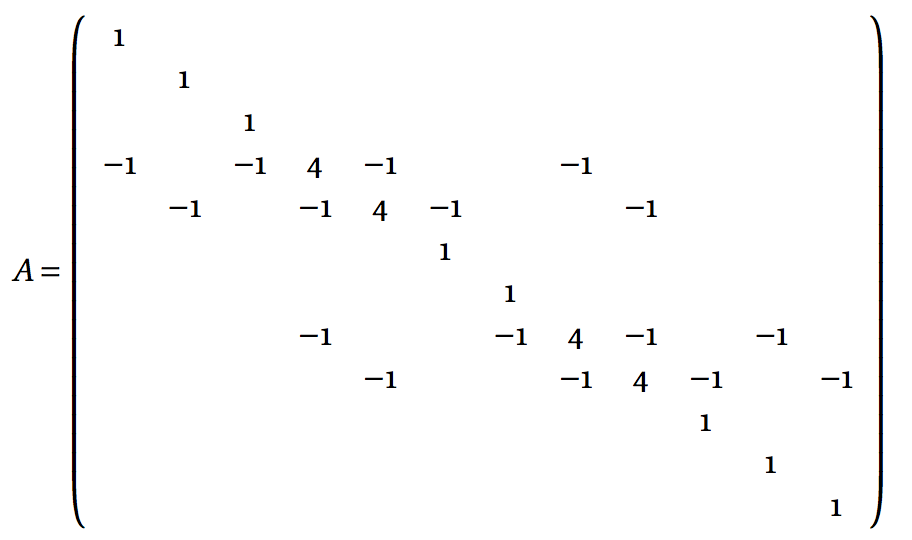
\includegraphics[scale=0.55]{ch2/8}
\end{center}

Notice that that the structure is not an upper or lower triangular structure and requires efficient solving methods. This is an equilibrium problem, in structural analysis Gaussian elimination is used but in fluid dynamics it is too costly and we use iteration methods. 

\subsection{Supersonic flow $M_\infty = \sqrt{2}$}
For supersonic case, we have an evolution problem and we have to specify $\phi, \frac{\D \varphi }{\D x}$ on the left boundary and one condition on the upper and lower boundaries, but no more at the outlet. Let's discretize the boundary points 1 and 2, we need external points a and b: 

\begin{equation}
\begin{aligned}
- \frac{\varphi _4 - 2\varphi _1 + \varphi _a}{h^2} &+ \frac{\varphi _2 - 2\varphi _1 + \varphi _c}{h^2} = 0\\
\Rightarrow \varphi _2 + \varphi _c - \varphi _4 - \varphi _a = 0 \qquad &\left.\frac{\D \varphi}{\D x} \right| _1 = \frac{\varphi _4 - \varphi _a}{2h} = u_1 \mbox{ (specified)}
\end{aligned}
\end{equation}

At this stage it is possible to eliminate the fictitious point $a$ using the derivative, same is done for point 2 in the second equation: 

\begin{equation}
-2\varphi_4 + \varphi_2 = - \varphi_c -2hu_1 \qquad -2\varphi_5 + \varphi_1 = - \varphi_d -2hu_2
\end{equation}

Grouping all together we again find a matrix: 

\begin{center}
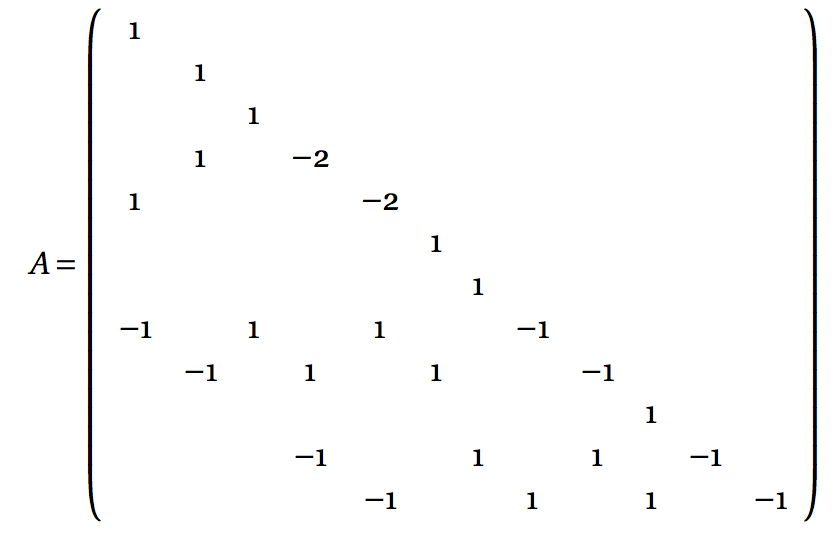
\includegraphics[scale=0.6]{ch2/9}
\end{center}

It is this time lower triangular and thus the solution is easily found by forward substitution. It is interesting to observe that the mathematical nature of the equation (marching in the zone of influence) is reflected in the method of solving (forward substitution). The problem of solving method does not arise here, the problem is the amplification of round off errors in the substitution process (stability of the method).

